The last day!

\subsection{Alan Wagner on Kantian One Day, Consequentialist the Next}

{\bf Main Idea:} Often faced with situations where you need to trade-off between different ethical frameworks. \\

Example: walking past a homeless person on the street. How do the particulars of that day effect whether you give aid to the individual or not? What about if the person is injured?\\

$\ra$ Previous psych study: participants were asked to attend an ethical symposium, along the way come across someone injured/in need. If the participant is in a rush, they tend not to help. \\

{\bf The Problem:} There is no agreed upon correct moral theory, and decisions vary by user and context. \\

Robotics community: tend to want robots that act ethically. \\

**Their approach: generate action recommendations for a robot based on several different ethical frameworks. \\

Method: survey different populations to see what they think are differen ethical actions (ask both average adults and ethics experts) \\

Three different ethical frameworks: 1) utilitarian framework focused on consequences, 2) Kantian framework focused on ethical duty, 3) social justice framework (fairness across groups), or 4) virtue ethics. \\

$\ra$ Focus on cases where these frameworks {\it disagree}. \\

$\ra$ Also, approach includes {\it moral emotions} like shame, pride, empathy, and so on. These emotions might effect whether a choice is ``right". \\

Q: So, what should a robot do? Let's say in the giving-aid-on-the-street case.\\

A: Form an action selection arbiter that takes as input suggestions for different ethical frameworks {\it and} contextualized model of human moral emotions (guilt, shame, pride, and so on). Pictured in Figure~\ref{fig:kant}. \\


\begin{figure}[h!]
\centering
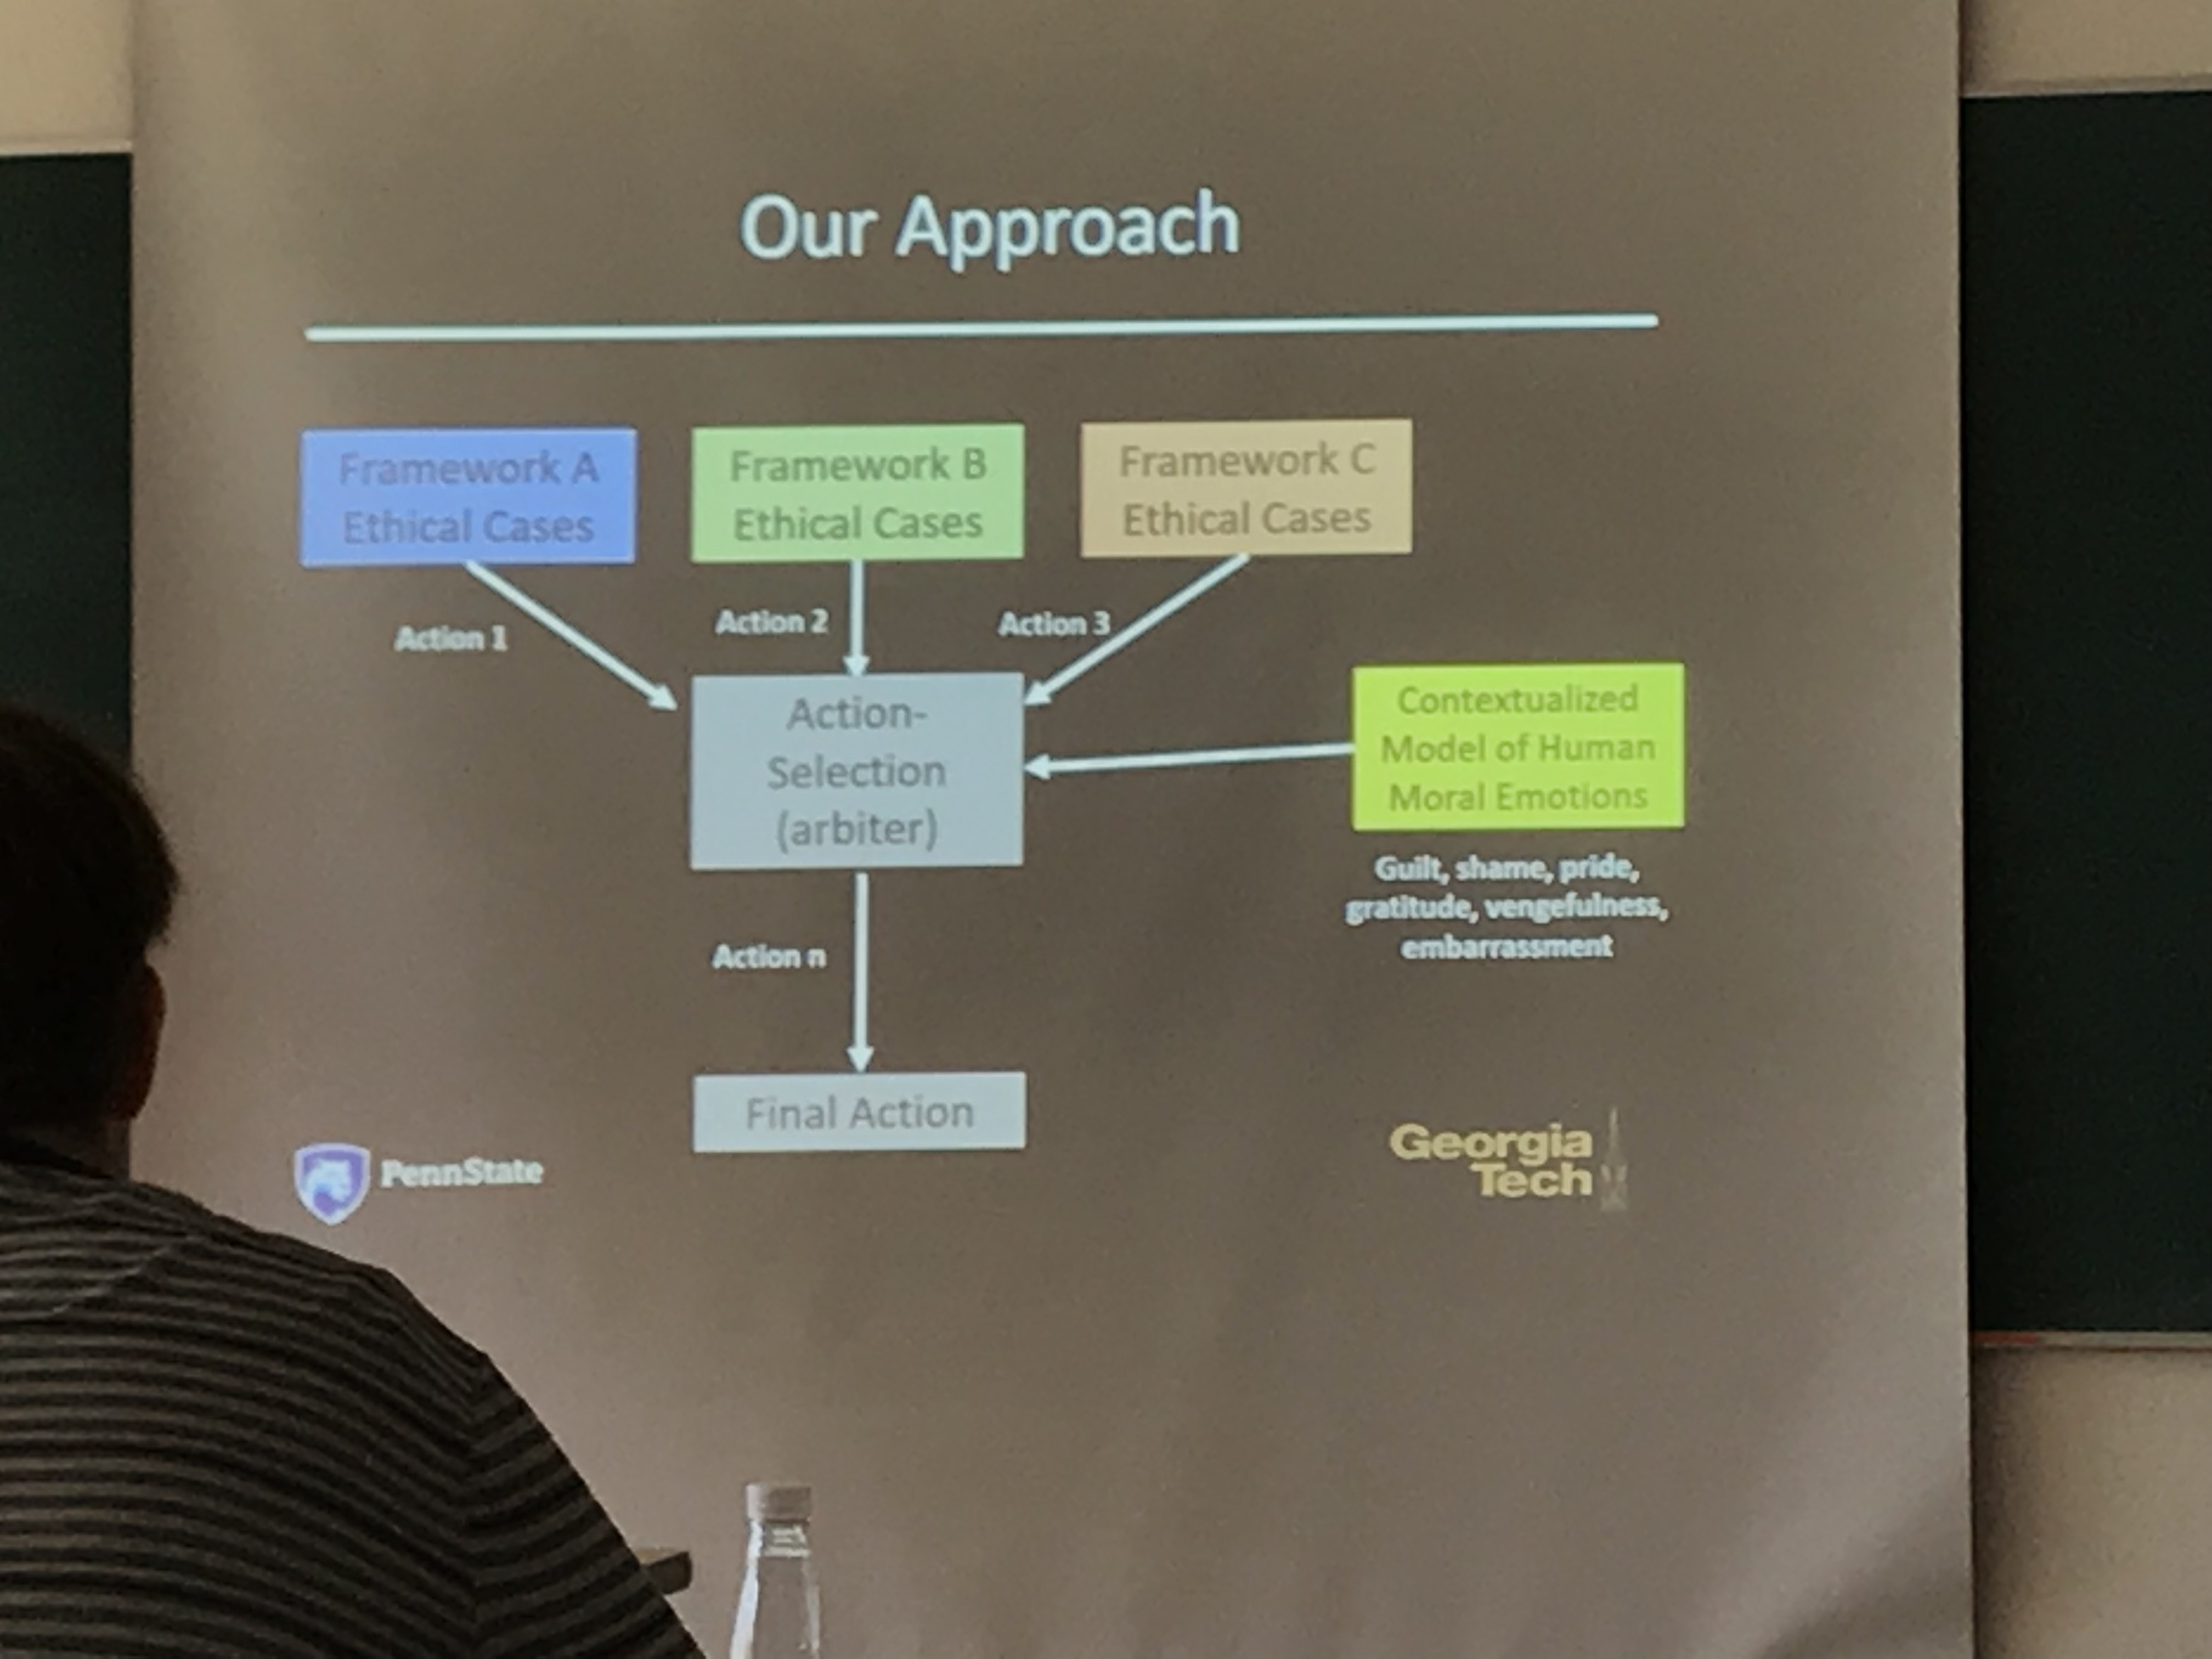
\includegraphics[width=0.5\textwidth]{kant.JPG}
\caption{Approach for ethical action arbitration and decision making.}
\label{fig:kant}
\end{figure}

{\bf Experiment 1:} Under which circumstances should one allow the opponent to win? Factors to consider: emotional state (is a child frustrated?), number of games played, age, others. \\

{\bf Experiment 2:} Pill sorting for elder care. Should the robot provide certain kinds of feedback? Say, false feedback that still encourages the person? \\


$\ra$ Survey for ethical ``answers": what do average everyday people say to do in these contexts (use AMT to collect data). Also collect ``expert opinons" from ethicists. \\


Contextualized Moral Emotions: robot retains model of emotional states of human participants; the models affect action selection. \\

Compare three action selection strategies:
\begin{enumerate}
\item Pill sorting: compare 1) always truthful (even when harsh), 2) Ethical expert recommendations, 3) Folk morality recommendations.
\item Game playing with children: 1) play to win, 2) ethical expert, 3) folk morality.
\end{enumerate}


Conclusions:
\begin{itemize}
\item Robot may need to use different ethical frameworks at different times.
\item These frameworks may not generate same action recommendations.
\item Robot may be able to use moral emotions to select best framework.
\item Possible trade-off between expert and folk opinions.
	\end{itemize}

\spacerule
\subsection{Angelica Fleury on Creating Moral Ideals in Robots from Buddhism}


{\bf Goal:} Introduce Buddhist principles for automated moral machines and contrast them from existing moral decision making methods. \\

Q: Can robots make moral decisions? \\

A: Amanda Sharkey in ``Can we program or train robots to do good?": she says no! Searle also would say no (via chinese room): strong AI can't understand their decisions, so can't make a moral decision. \\

Against Robot-Morality Skeptics:
\begin{itemize}
\item Require an assumption about a metaphysical ``self" tied to understanding. Necessary components for understanding morality.
\item Humans have a self, and this is typically sought after in robot design.
\item We ought to build a moral machine as nearly human as possible, requires claims that humans are the moral standard.
\item Objections; need for inner self as a basis for agent to have capacity fo be moral might be mistaken! Also, we should take into consideration disputes on the need for a metaphysical self.
$\ra$ Buddhists challenge the ethics of the self as something to be sought after.
\end{itemize}


Q: Should humans serve as a moral standard? \\

A: Might be the right starting point to model moral machines after, but not the standard. Our own agenda allows us to act selfishly (according to most ethical frameworks). \\

{\bf Objective:} Not to create a metaphysical moral criteria outside human influence, but instead to progress towards understanding how to make a moral machine. \\

Q: What are the necessary components for a Budhist-influenced AMA?

A: (from Danstini, Floor, Meyer 2006): 1) Autonomy (minimal sense, not Kant), 2) Emotions (need to be reciprocal, guide expression and motivation), and 3) Emotion regulation (maintain desirable emotions). \\

{\bf Approach 1:} program agents with emotions via BDI-Based agent programming language. \\
{\bf Approach 2:} program agents with emotions via ALMA (a layed model of affect). \\

$\ra$ Suggestions for modifying agents with emotions: 1) Programin initial mood to maximize empathy, 2) Appraisal (less reactionary, motivated by compassion), and 3) Coping with artifical emotion (their still triggered by if-then statements, human understandable). \\

{\bf Example:} Patient with dementia who is in need of assistance, but providers are reluctant to interact with patient due to emotional distress. Provider may neglect necessary interactions, whereas a moral machine can take into account negative emotions and recognize the need for interation and its negative emotions can be overriden. \\

Conclusions:
\begin{itemize}
\item Don't get too hung up on metaphysics of self
\item Reconsider that moral machines need to be just like humans
\item Keep emotions around but use mindfulness as a model to incorporate emotion.
\end{itemize}

\spacerule
\subsection{Simon Award Talk: Juan M Dur{\' a}n on Philosophically Analyzing Simulations}

{\bf Focus:} Come up with a systematic approach for studying computer simulations from a philosophical perspective (concentrating on two viewpoints). \\

Outline:
\begin{enumerate}
	\item First viewpoint: Problem-solving technique viewpoint
	\item Second viewpoint: Description of patterns of behaviour viewpoint: 1) historical definitions (1960-2013), 2) common topics, 3) philosophical assumptions.
	\item Philosophical implications/studies of computer simulations.
\end{enumerate}



\subsubsection{View 1: Problem Solving Techniques (PST)}

{\bf Idea:} Computer simulations are about solving a problem. \\

\ddef{PST (take one)}{(Teichroew and Lubin 1966) ``Simulation problems are characterized by being mathemaically intractable and having resisted solution by analytic methods"}

\ddef{PST (take two)}{(Humphrey 1990): ``A computer simulation is any computer implemented method for exploring the properties of mathematical models where analytic methods are unavailable."}


Common Themes from PST definitions: 1) Simulations are about finding the set of solutions to mathematical models, 2) Use of simulations is justified when analytic methods are unavailable, and 3) exploring {\it properties} of mathematical models. \\


%\subsubsection{Philosophical Assumptions}

Three key assumptions (for when to use computational simulations according to PST):
\begin{enumerate}
	\item Analytic intractibility

	$\ra$ Simulations are a tool for computing. Instrumentral role for finding results for a model. Understood as epistemically inferior to analytic methods.

	\item Implementation {\it simpliciter}

	$\ra$ Assumed that mathematical models can be directly implemented as a computer simulation. No genuine methodology mediates between the models and simulation.

	$\ra$ Simulation models are ontologically on par with mathematical models.

	\item Inherited representational capacity

	$\ra$ Simulations inherit their representational capacity of a target system from the mathematical model they implement.
\end{enumerate}

Recent paper from Bueno and Colyvan (2014) high {\it representation} as a critical piece of theories of computer simulations.

\subsubsection{View 2: Description of Patterns of Behavior (DPB)}

Again, a historical recorrd;

\ddef{DPB (take one)}{(Shubik 1960): `a simulation of a sytem is operation of a model or simulater which is the representation of a system}
\ddef{DPB (take two0}{(Bristwitle 1980) ``Simulation is a technique for representing a dynamic system by a model in order to gain information about the underlying system".}
\ddef{DPB (take three}{(Shannon 1998): ``The process of designing a model of a real system and conducting experiments with this model for the purpose of understanding the behavior of the system and evaluating various strategies for the operation of the system."}


Main idea: simulations are units of analysis in their own right (in the same way that scientific tests are). \\


Commonalities across these definitions: 1) Computer simulatins are primarily concerned with descriptions/representations of the target system, and 2) Simulations allow inferences about properties of the target system. \\


Three key assumptions (for when to use computational simulations according to DPB):
\begin{enumerate}
\item A proper methodology for computer simulations.

	$\ra$ Computer simulations become units of analysis in their own right. 

\item Own/proper representational capacity of the simulation.

\item New forms of knowledge.

	$\ra$ Capable of giving rise to new knowledge that we couldn't access through other means.
	\end{enumerate}



\subsubsection{Philosophical Implications}

Q: What can we learn about scientific explanation from these views of computer simulation? \\

A (Traditional view): mathematical model can give explanation for real-world phenomena, but not necessarily computer simulation (view from Kros 2008, Weirich 2011). \\

$\ra$ Scientific explanation: ``Simulation model does not provide an acceptable explanation of the material system" (Krohs 2008). \\

Explanation for the PST:
\begin{itemize}
	\item Analytic Interpretability
	$\ra$ ``Theoretical models need to be further analyzed or solved to provide descriptions of and predictions about the dynamics of the world they model." (Krohs).
	\item Implementation {\it simpliciter}
	\item Inherited representational capacity
	$\ra$ Since the simulation does not have explanatory input on its own and since it is limited to relating the theoretical model with the realworld phenomena, the simulation must inherit the representational capacity of the mathematical model.
\end{itemize}

Q: Do computer simulations have more to say about explanation? Or is that it? (the PST story) \\

A: Yes, explanation is better understood through the DPB \\

** Better view (from the DPB): When we explain, we don't explain the real world, {\it we explain the results of a simulation} (and hope the simulation is linked to the real world). \\

$\ra$ To solve this explanatory difficulty, we can draw a distinction between {\it knowledge} and {\it understanding}. Explanations can give us {\it understanding}, but not knowledge. \\

Key Idea: results actually shed light on the simulation itself; they help us {\it understand} the simulation. \\


Explanation for the DPB:
\begin{itemize}
	\item Scientific explanation: ``It is the simulation model, and not an exogenous mathematical model, the unity with the most explanatory relevance for the results of the simulation" (Dur{\' a}n 2017).
	\item A property methodology for computer simulations
	$\ra$ Simulations must be units of analysis in their own right.
	\item Self representational capacity of the simulation
	$\ra$ It makes possible the didentification of what can be ascribed to the world and what is an artifact of the simulation
	\item New forms of knowledge
	$\ra$ computer simulations have a {\bf genuine explanatory role} and thus ground their epistemic power.
\end{itemize}


\subsubsection{Conclusions}

Recap: two distinct viewpoints on computer simulations and their role in scientific explanation. \\

$\ra$ PST and DPB are two different theoretical frameworks about the philosophical study of simulation. PST strongly depends on mathematical models, where DPB view suggest a new methodology and epistemology of computer simulations. \\


Important note: not all definitions qualify as PST or DPB (though these two comprise most of the literature). Some others: 1) Computer simulations are arguments (Beisbart 2012), 2) COmputer simulations as unfolding the content of a well-described scenario (El Skaf, Imbert 2013). \\

Conclusion: if we can come up with well established views that unify perspectives/definitions, we can take ourselves further in this literature.

\spacerule

\subsection{Alan Wagner on The Aristotelian Robot}

{\bf Focus:} Philosophical treatment of a what it would look like to construct an Aristotelean robot. \\

$\ra$ Guiding Q: How can we construct a robot that can make use of virtue ethics? \\

$\ra$ Virtue ethics focuses on the agent, while deontology focuses on the maxim that oreitns moral action, and uitilitarian theories focus on outcomes. \\

{\bf Central Claim:} Aristotelian ethics is an optimal framework to implement for an artificial social agent. Reasons:
\begin{itemize}
	\item It can be implemented as a moral learning framework
	\item It can take into account moral psychologcal and the role of moral emotions.
\end{itemize}
%\ddef{Virtues}{Virtue is a state concerned wth choice.}

Q: Are humans by nature moral? \\
A: No! We {\it learn} to be educated by our community and our experiences. we are ``Aristotelian" humans first, later we may become Kantian, utilitarians, or nihilists. At first we are taught virtues using moral narratives and engaging their moral emotionds (moral pedagogy through narration can help teach us about morality!). \dnote{I remember reading the book of virtues as a kid!}\\

Q: How did humans become moral? \\

A: societal pressures and evolution generated the conditions for morality. Moral emotions played a critical role. \\

***Morality is a {\it societal accomplishment}. \\

Agents can learn to be moral by interacting with a community: virtues are embedded in the community. \\

Aristotle claim: core virtues are {\it quasi-universal}, and should appear in most groups: 1) self-respect, 2) gratitude, 3) courage. When a {\it conflict} arises among exemplars, core virtues are engaged. \\

$\ra$ Moral conflict can cause reflection/introspection: why is something important? Social conventions/norms unburned us from constrant moral reflection. \\

Q: How do we train a moral robot? \\

Approach: use moral narratives to teach!
\begin{enumerate}
	\item Traditionally moral training takes the form of narratives: Odysseus, Mulan, the Bodhisattva in the Jatakas.
	\item Consider the hypotheticals: ``What should X do in this situation?".
	\item Challenge: using narratives in this way requires emotional understanding!
\end{enumerate}


Aristotetlian Framework:

%\begin{figure}[h!]
%\centering
%\includegraphics[width=0.5\textwidth]{ari.JPG}
%\caption{The Aristotelian Framework}
%\end{figure}

Questions Considered:
\begin{enumerate}
	\item Are we intrinsically moral?
	$\ra$ No
	\item Moral pedagogy $\ra$ Aristotelian model
	\item Does reason move us to morality?
	$\ra$ No
	\item Can we be moral without a sense of moral persona?
	$\ra$ No
	\item Did we make ourselves moral?
	$\ra$ Yes
	\item Does the moral ``I" depend on moral narratives?
	$\ra$ Yes
	\item Does reason depend on affect to tell us what is moral?
	$\ra$ Yes
	\item Feelings required for moral emotions
	\item What's the role of phenomenology in morality?
\end{enumerate}


Conclusion:
\begin{itemize}
	\item Should be post-Cartesian and post-Turinian; we need to connect mind and body and recognize the importance of narrativity in morality.
	\item Just having emobdiment is not ehough.
	\item Cannot separate emotions from emodiement.
	\end{itemize}


\spacerule

\subsection{Himavath Jois on Should Robots be Allowed to Punish Us?}

{\bf Scenario:} an elementary school sets up a mixed robot/student team to build a bridge. In a typical team, if a student misbehaves, the teacher might scold them (put them in time out, etc.). But in this joint robot-student team, should a robot be allowed to put a misbehaving student in timeout? \\

\dbox{Guiding Q: Should robots be allowed to punish people in some circumstances?}

``Humans tend to cede decision making authority to machines in mixed robot-human teams" (Gombolary et al.). \\

Q: What is punishment for? Why is it necessary? \\

A: Punishment is critical for teaching! (See: education, sports, norms)---especially when mistakes are costly (military). \\

Q: Will humans accept punishment from a robot? And in particular, how will people respond? \\

Naive Hypothesis: People will prefer to be punished by a ronot (not advocating for this, but speculating), even when the punishment is physical! \\

Experiment: explore whether this hypothesis has merit. Setup involves a punishment device: a robotic exoskeleton capable of physical restriction as punishment for a wearer's action. \\

$\ra$ Key ethical frameworks: consequentialism, conserving autonomy, utilitarianism. \\

\begin{itemize}
	\item Consequentialist view: if the punishment leads to decreased wrongdoing, we might view it as a good thing (but, we have to consider the decrease in autonomy/pleasure of the individual)
	$\ra$ Toward autonomy: Bentham's Panoptican. Too much surveillance decreases autonomy. Would we prefer emotional control or physical control? Or just object to this loss of autonomy?

	\item Utilitarianism vs. Retributivism: Goal is to administer a punishment that decreases crime/wrongdoing. Retributive would be eye-for-an-eye.

\end{itemize}

Three scenarios:
\begin{enumerate}
	\item Scenario 1: A new house arrest device allows prisoners to live outside of prison but limits what they can do.
	\item Scenario 2: An army uses exoskeletons to maintain control over recently surrendered soldiers.
	\item Scenario 3: A world leader uses robotic exoskeletons to control a civil population and limit unrest.
\end{enumerate}

In light of these scenarios, conduct experiments that vary the type of punishment on individuals. Can receive any of: 1) no punishment, 2) verbal scolding, 3) physical restriction (through the exoskeleton). \\

$\ra$ Contrast a human initiator vs. a robotic initiator (for the punishment). \\

{\bf Preliminary Results:}
\begin{itemize}
	\item Pilot subjects presented with Godspeed survey:
	$\ra$ reported that physical punishment was very frustrating
	$\ra$ subjects that underwent robot initatied punishmen found the exoskeleten more intelligent than the human
	\item Minimal understanding of subject preferences
	\item Motivating subject to trade accuracy for speed is difficult.
	$\ra$ Currently in the process of reivisitng the methodology
	$\ra$ So this is the only beginning (but again: we're not advocating for this to happen). Just want to initiate the academic conversation, better understand human preferences about these topics.
\end{itemize}

Q: Why should we even think about this?
A: ``The machine does not isolate man from the great problems of nature but plunges him more depliny into them", Antoine de Saint-Exupery in {\it The Little Prince}. \\



\spacerule{}

\subsection{Presidential Address: Don Berkich on Underdetermination after Computation}


Q: should the philosophy of science community catch up to new computational methods? Do philosophers of science care about these advances?  (they should!) \\

\ddef{Naive View of Science}{A theory proposes (in the strong deductive sense), an experiment disposes}

One try: Observation $\implies$ $\neg$Hypothesis. But that can't be right. ``Observation" isn't propositional. \\

Note: really want to understand what we mean by ``observation" in the computational age. \\

Second try: ExperimentalObservation $\implies$ $\neg$Hypothesis. Where, ``ExperimentalObservation" is the proposition that ``specific states of affairs incompatible with the truthe of hypothesis have been experimentally observed to obtain." \\

Q: Why is this naive view of science naive? \\

A1: ExperimentalObservation is ``theory laden" (see: Duhem 1906 and Quine's Two Dogmas 1951). No putatively observational statement is observational. %Empiricists insistence on the truth of synthetic statements being reducible to the emnpirical conditions of their verification is no more sensible than their insistence that the truth of analytic statements is solely via the relationships between the meanings of terms in the statements.


A2: If ExpObs is theory laden, then falsification is ambiguous. \\

A3: If falsification is ambiguous, then scientific theory is underdetermined by the evidence for it (see: Duhemian Holism or Quinean Holism). \\

A4: Is scientific theory is underdetermined by the evidence for it, then there are no ``crucial" experiments in science. \\

A5: If no crucial experiments, then theory choice is determined by extra-scientific values.

\dbox{$\therefore$: Theory choice is driven by extra-scientific values.}

Q: What are the extra-scientific values in question? \\

Duhem A: Experimenter must display ``good sense" in choosing theory. \\

Quine A: Scientists may appeal to such principles like minimal mutilation that tend to protext math and logic. \\

$\ra$ Upshot: By good sense/minimal mutiliation/other values, naive view of science is naive insofar as it ignores the necessary role of these values in theory choice. \\

Holism: hypotheses are affected by: Science {\it and} math {\it and} Logic {\it and} Computability. \\

Q: How does the widespread deployment in the service of science affect Duhem and Quine's accounts? \\

Examples of computational methods used in science (on the side of the entailing proposition in the naive view): hurricane modeling, cellular modeling, neural modeling, ecological systems, and so on. \\

$\ra$ Computer modeling/simulations are just one half of the computational turn in the sciences. We also have data collection. \\

*These pieces are so powerful, we should update the view of science to: ComputationalObservation $\implies$ $\neg$ Hypothesis, where CompObs is the proposition that ``specific states of affairs incompatible with the truth of Hypothesis have been algorithmically inferred from vast data-troves automatically collected and classified from multiplicities of sensors. \\

Q: What is the observation when perceptual experience is no part of CompObs?\\

Discussion: Is CS epistemically privileged? Thinking about Quine's implicative view, is CS distinct from math/logic/science in some sense? \\

$\ra$ View 1: CS is science, enjoying no greater privilege than the rest of science.
$\ra$ View 2: CS is like math/logic, epistemically privileged either by being {\it a priori} or defensible as occupuyng a central commanding position in our web of belief. \\


{\bf Conclusion:} Wanted to ask: how does CS factor into our scientific theory? Is it epistemically privileged in some sense? Each possibility visited represents trouble. Moreover, computationall mediated observation may turn out to be a shaky foundation on which to build the edifice of science (as we're doing).


\dnote{And that's a wrap!}
\spacerule








